\documentclass[12pt, english]{beamer}

% Packages
\usepackage{xcolor}
\usepackage{eulervm}
\usepackage[utf8]{inputenc}

% Theme
\mode<presentation>
{
  \usetheme{Honefoss}
  \setbeamertemplate{blocks}[rounded]
}

\newcommand{\comment}[1]{{\slshape\color{kvred}#1}}

\title{Where}
\subtitle{A Geodetic Software}
\author{Ingrid Fausk, Michael Dähnn, Ann-Silje Kirkvik}
\date{April 6, 2019}

\begin{document}
\frame[plain]{\titlepage}

\begin{frame}{Where Timeline}
  \begin{itemize}
    \item 2015: Start
    \item 2018: First release as an open source project on GitHub
    \item 2019: Two proposed IVS analysis centers with Where: 
       \begin{itemize}
         \item Kartverket, Norway
         \item Instituto Geográfico Nacional, Spain
       \end{itemize}
    \item 2020: IVS Analysis centers with Where?
    \item 2022: ILRS Analysis center with Where?
  \end{itemize}
\end{frame}

\begin{frame}{Live Demo of Where}
  \begin{itemize}
    \item Running \emph{Where}
    \item Running \emph{There}, a companion tool for visualizing results
    \item Status, discussion
    \item Bugs...
  \end{itemize}
  \begin{figure}
    \begin{flushleft}
      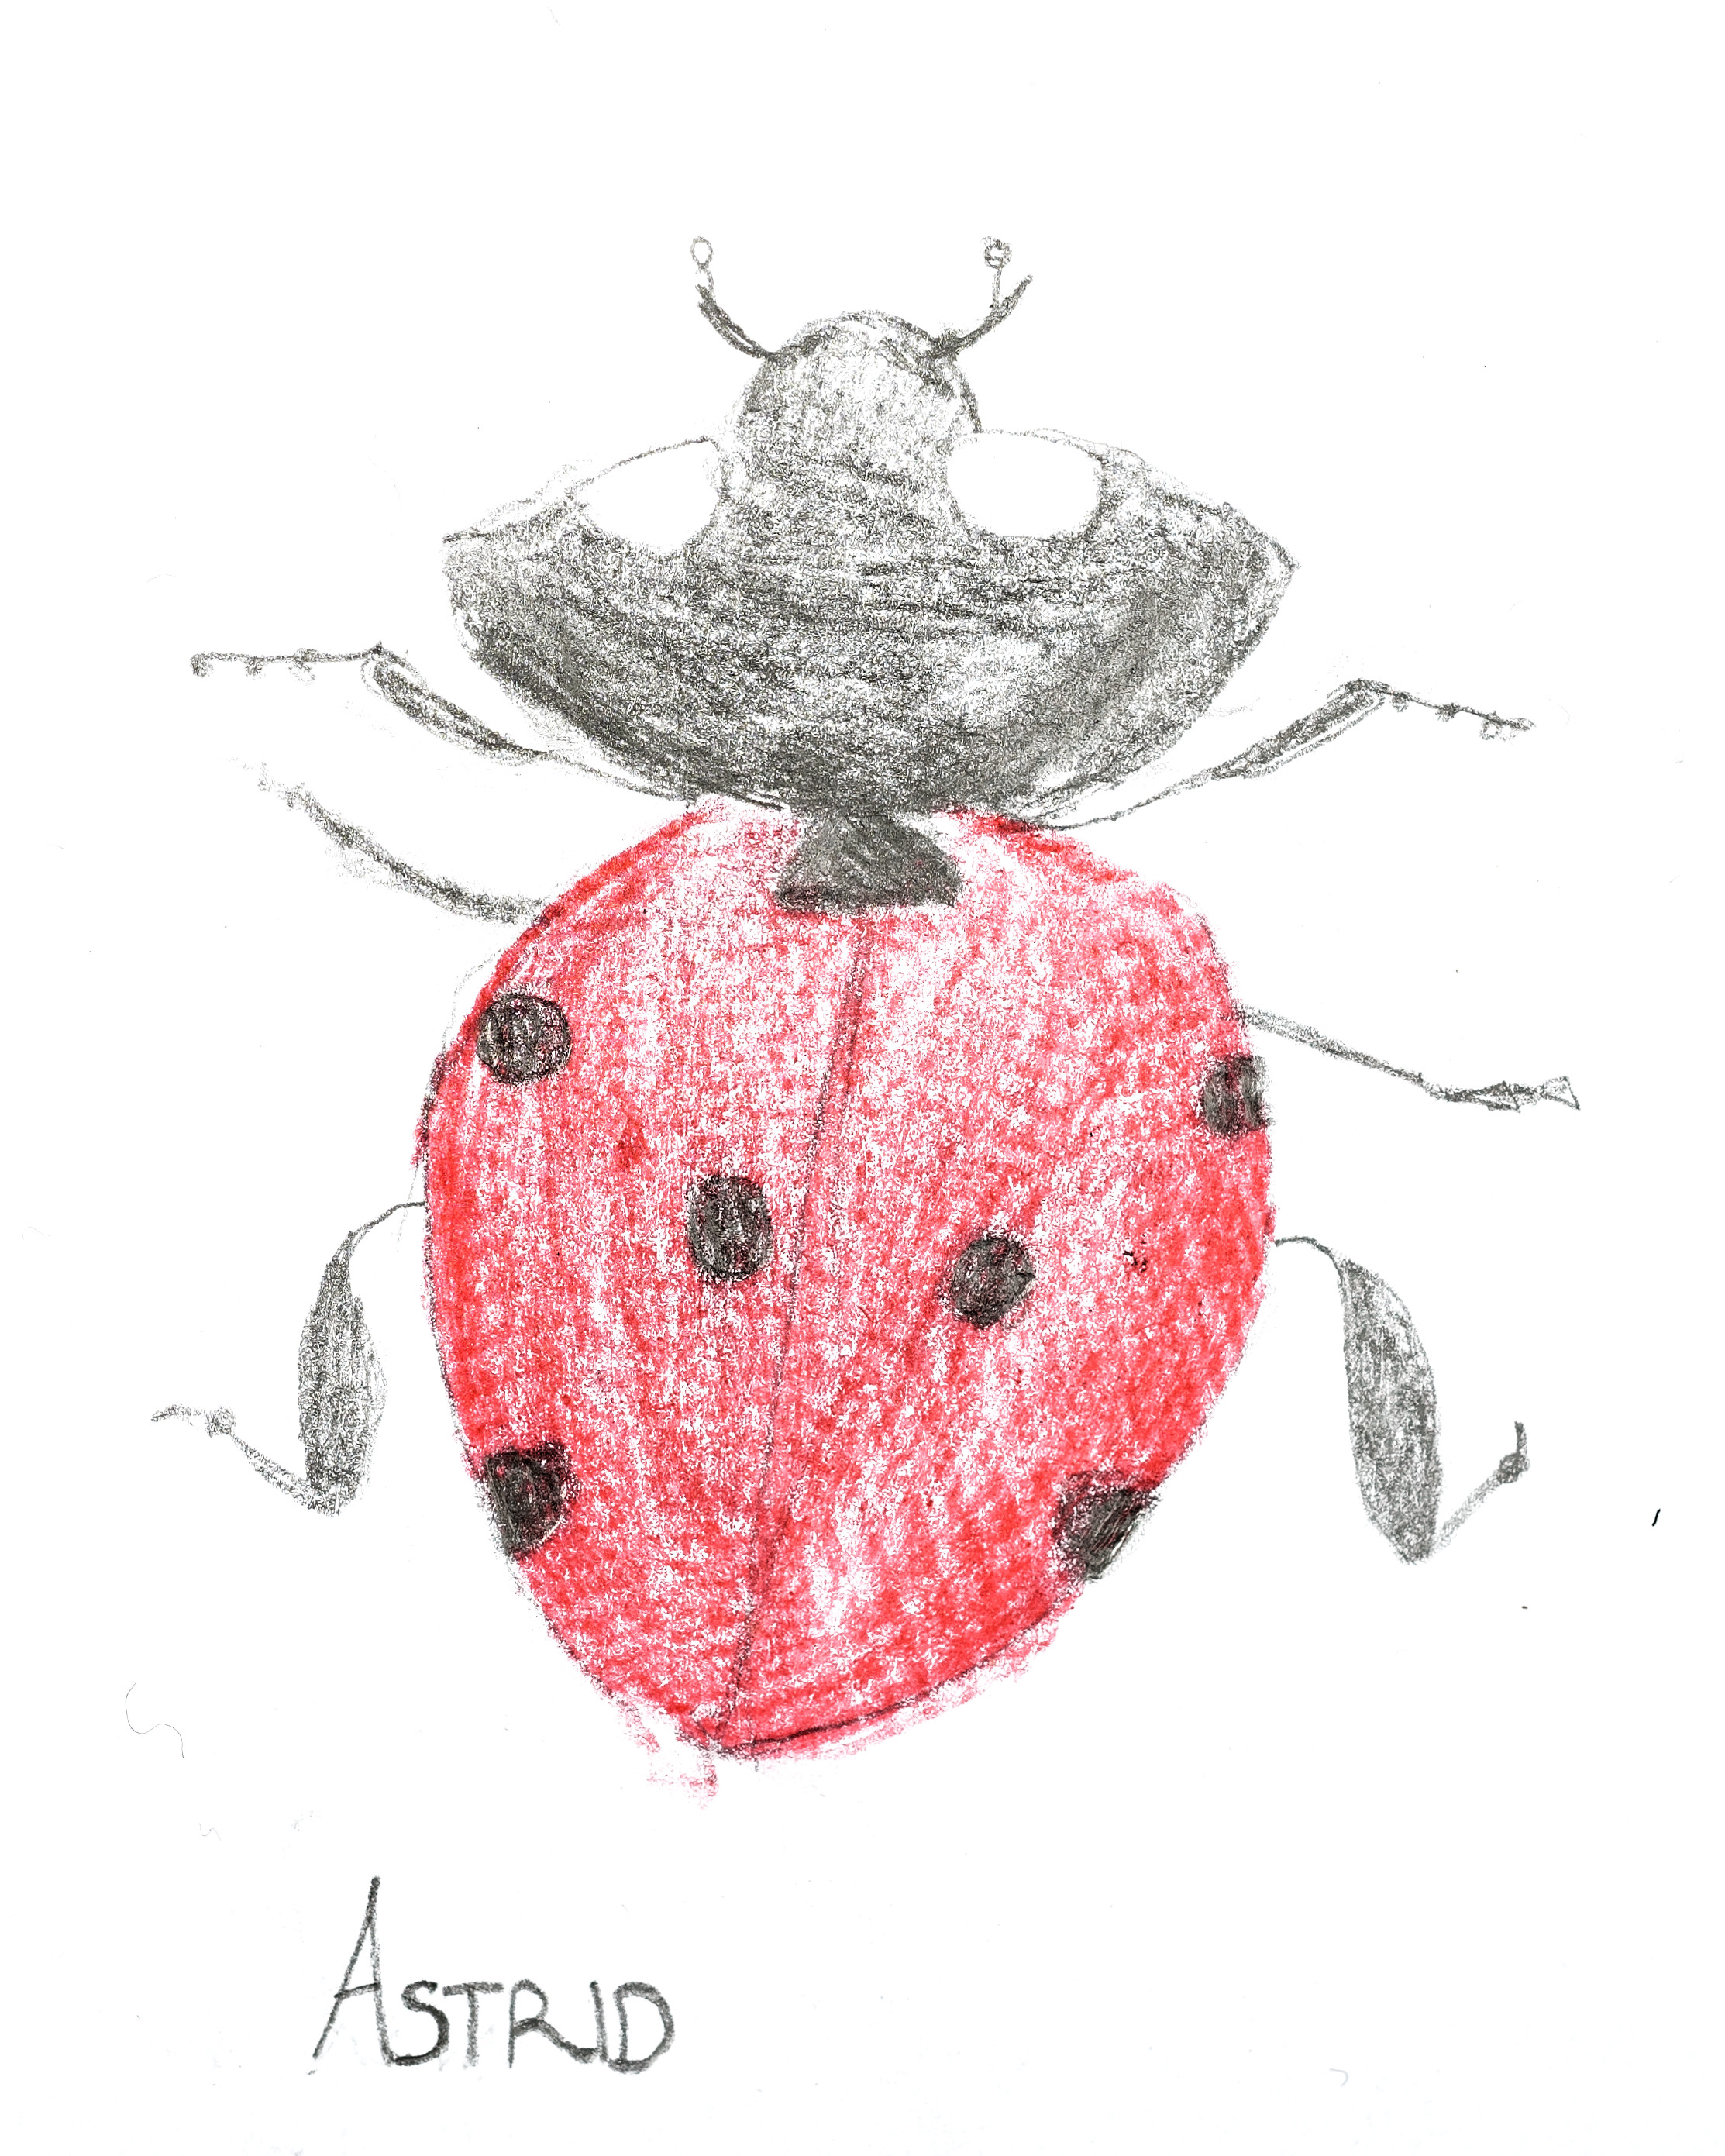
\includegraphics[width=2.5cm]{bug.jpg}
    \end{flushleft}
  \end{figure}     
\end{frame}

\begin{frame}{The Technical Stuff}

The \textbf{Where} software is mainly being written in \emph{Python}

  \begin{itemize}
    \item Cross-platform: Runs on Linux, Mac, Windows
    \item Solid, flexible and fast libraries like \texttt{numpy}, \texttt{astropy}, \texttt{matplotlib} and \texttt{scipy} are available
    \item We use a \textbf{HDF5}-based format for internal data storage
    \item \emph{Python} has effective interfaces to \emph{C} and \emph{Fortran} code, and we use the \textbf{SOFA} and \textbf{IERS} software libraries directly
    \item Orbit integrator using \emph{Cowell} method written in \emph{Python}. 
  \end{itemize}
\end{frame}

\end{document}
